%% Estructura principal para un reporte de Trabajos intersemanales CIRCAE %%
\documentclass[a4paper]{IEEEtran} %tamaño del papel y el tipo de transcripción que será IEEE
\usepackage[utf8]{inputenc} %el tipo de codificación que incluye símbolos como la tilde
\usepackage[spanish]{babel} % hacemos que nuestro documentación vaya en español
\usepackage{cite} % citas bibliográficas
\usepackage{graphicx} %gráficos, usaremos solo .jpg o .png con estándares que ya veremos
\usepackage{subfigure} %usar subfiguras
\usepackage{url} %agregar direcciones url
\usepackage{amsmath} %expresiones matemáticas
\newtheorem{teor}{Teorema}[section] %definimos la enumeración de Teoremas usando la etiqueta \begin{teor} ... \end{teor} para los ejemplos, podemos darle etiquetas para referenciarlas a lo largo del texto
\newtheorem{ejem}{Ejemplo}[section] %definimos la enumeración de Ejemplos usando la etiqueta \begin{ejem} ... \end{ejem} para los ejemplos, podemos darle etiquetas para referenciarlas a lo largo del texto
\newtheorem{exper}{Experimento}[section] %definimos la enumeración de Ejemplos usando la etiqueta \begin{exper} ... \end{exper} para los Experimentos, podemos darle etiquetas para referenciarlas a lo largo del texto
\usepackage{setspace} %LA usamos para asignar el interlineado
%%%%%%% settings para incluir codigo fuente en cualquier lenguaje
\usepackage{listings} %comenzamos la configuración de nuestras lineas de codigo que se incluirá de ser necesario en el documento
\usepackage[usenames]{color} %seteamos el uso de nombre y color
\definecolor{gray97}{gray}{.97}%definimos nombre y color
\usepackage{textcomp}
\lstset{
		frame=Ltb,
		framerule=1pt,
		framextopmargin=5pt, %margen de arriba
		framexbottommargin=5pt, %margen de abajo
		framexleftmargin= -2pt, %separacion del margen izquierdo
		framesep=2pt,
		rulesep=0.2pt,
		backgroundcolor=\color{gray97},
		rulesepcolor=,
        tabsize=4,
        rulecolor=\color[RGB]{106, 182, 217}, %AZUL
        upquote=true,
        aboveskip={1.5\baselineskip}, %despues de la linea de texto
        columns=fixed,
        showstringspaces=false,
        extendedchars=true,
        breaklines=true,
        prebreak = \raisebox{0ex}[0ex][0ex]{\ensuremath{\hookleftarrow}},
        showtabs=false,
        showspaces=false,
        showstringspaces=false,
        basicstyle=\scriptsize\ttfamily\color[RGB]{39, 100, 46}, %Numeros de lineas, simbolos, puntos y coma y demas
        identifierstyle=\ttfamily\color[RGB]{56, 140, 189}, %variables
        commentstyle=\color[RGB]{62, 179, 101}, %comentarios
        stringstyle=\color[RGB]{247, 165, 42}, %impresiones
        keywordstyle=\bfseries\color[RGB]{237, 118, 150}, %funciones
        %
		numbers=left,
		numbersep=-7pt, %separacion del numero
		numberstyle=\tiny,
		numberfirstline = false,
		breaklines=true,
		}
\usepackage{graphicx}
\usepackage[colorinlistoftodos]{todonotes}
%%%%%%%
\providecommand{\keywords}[1]{\textbf{\textit{Términos Clave---}} #1}

\begin{document}
\spacing{0.9} %definimos un interlineado de 0.9 para todo el documento

\title{Nombre del Proyecto en Puestión}
\author{NombreA1 ApellidoA1 ApellidoA2, Miembro, CIRCAE, NombreB1 ApellidoB1 ApellidoB2, Miembro, CIRCAE
\thanks{Este primer párrafo puede contener auspiciadores u organizaciones que colaboraron con la realización de esta parte del proyecto y mencionar de manera expecífica que papel puntual tuvieron en el proceso... "This work was supported in part by the U.S. Department of Commerce under Grant BS123456."}
\thanks{Los siguientes párrafos pueden contebner datos específicos de los autores del proyecto, por ejemplo "F. A. Author is with the National Institute of Standards and Technology, Boulder, CO 80305 USA (e-mail: author\@ boulder.nist.gov)"}
\thanks{NombreA1 ApellidoA1 ApellidoA2, was with Rice University, Houston, TX 77005 USA. He is now with the Department of Physics, Colorado State University, Fort Collins, CO 80523 USA (e-mail: author\@ lamar.colostate.edu).}
\thanks{NombreB1 ApellidoB1 ApellidoB2 is with the Electrical Engineering Department, University of Colorado, Boulder, CO 80309 USA, on leave from the National Research Institute for Metals, Tsukuba, Jaan (e-mail: author\@ nrim.go.jp).}}

\markboth{CIRCAE INFORME \today -G1-P3-005}{} % Codigo del informe que corresponde a: - numero de grupo con la G antepuesta - numero de proyecto con la P antepuesta | número de informe
\maketitle


\begin{abstract}
MicroMouse es un dispositivo en el que se aplica principios de ciencias de la computación, principios ópticos, mecánicos, electrónicos y la integración de tecnologías de software y hardware  . Lo que se pretende cubrir es la solución de un laberinto usando algoritmos de reconocimiento, almacenamiento, solución y retroalimentación con condiciones iniciales constantes en el tiempo.\\

\keywords{\textbf{Introducimos nuestros términos clave en orden alfabetico, separado por comas. Para una lista de sugerencias de palabras o términos clave visitar \underline{http://www.ieee.org/organizations/pubs/ani\_ prod/keywrd98.txt}}}
\end{abstract}

%%%%%%%%%%%%%%%%%%%%%%%%%%%%%%%%%%%%%%%%%%%%%%%
%%%%%
%%%%%   PROBLEMA     %%%%%%%%%%%%%%%%%%%%%%%%%%
%%%%%
%%%%%%%%%%%%%%%%%%%%%%%%%%%%%%%%%%%%%%%%%%%%%%%

\section{Problema}
\label{problema} %Tambien se puede poner etiquetas a secciones, subsecciones, subsubsecciones

El problema será planteado con un pequeño preambulo y luego enumerado con items de la siguiente manera:

    \begin{itemize}
    	\item Este es la primera parte del problema
    	\item Segunda parte del prblema, y se puede saltar al siguiente sin necesidad de agregar barras ivertidas %estos --> \\
		\item Tercer item tambien importante, y así se púede agregar más items al problema
	\end{itemize}

	Otra manera de agregar partes del problema es enfatizando algunas palabras, usándolo de la siguiente manera:

	\begin{itemize}
		\item \textbf{Interferencia} que nos lleva a la descripción del problema relacionado con interferencia.
		\item \textbf{Ahorro energetico} en los circuitos en la fase de prototipado, que por lo general tienen un alto consumo energético.
	\end{itemize}

El uso de los items no es necesario si se tiene bien definido solo un punto, o dos, los cuales pueden ser abordados en un solo párrafo, o en más de ser necesarios, para ello siempre haremos uso de las dos barras invertidas\\ % estos --> \\
Como se podrán dar cuenta, si incluimos estas dos barras, y solo saltamos un renglon, tendremos este resultado pero si incluimos las dos barras y luego saltamos un renglon como sigue \\

Tendremos este resultado, un párafo que tiene indentación, mientras que el anterior no lo tiene, tampoco tiene el espacio entre párrafo y párrafo extra.

Tendremos este resultado, un párafo que tiene indentación, mientras que el anterior no lo tiene, tampoco tiene el espacio entre párrafo y párrafo extra.
Tendremos este resultado, un párafo que tiene indentación, mientras que el anterior no lo tiene, tampoco tiene el espacio entre párrafo y párrafo extra.

Tendremos este resultado, un párafo que tiene indentación, mientras que el anterior no lo tiene, tampoco tiene el espacio entre párrafo y párrafo extra.
Tendremos este resultado, un párafo que tiene indentación, mientras que el anterior no lo tiene, tampoco tiene el espacio entre párrafo y párrafo extra.

Tendremos este resultado, un párafo que tiene indentación, mientras que el anterior no lo tiene, tampoco tiene el espacio entre párrafo y párrafo extra.

De ser necesario se podría incluir algun gráfico pequeño, teniendo en cuenta que el máximo en ancho de imagen será de $8.5cm$ como se muestra en la figura \eqref{img1}, tomar este dato con cautela, ya que gráficos como una captura de pantalla no podrán mostrar toda su informacion en 8.5cm de ancho.

\begin{figure} %Comenzar la figura
    \centering %hacemos que la imagen en cuestion esté centrada, si guera de 5 o 6 cm, esta se vea bien
        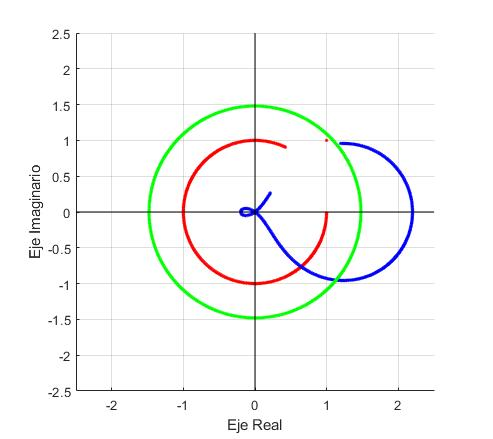
\includegraphics[width=8.5cm]{imagenes/img1} %incluimos la imagen con una característica especial: la medida definida en centímetros e incluimos la ruta de imagen sin especificar la extensión de la imagen (solo usaremos .png y .jpg)
        \caption{Un gráfico de Matlab} %La descripción de la imagen, ser concisos
        \label{img1} %La etiqueta usada para poder referenciarla desde cualquier parte del texto como se hizo con /eqref{img1}
\end{figure} %finalizamos la figura

%%%%%%%%%%%%%%%%%%%%%%%%%%%%%%%%%%%%%%%%%%%%%%%
%%%%%
%%%%%   OBJETIVOS     %%%%%%%%%%%%%%%%%%%%%%%%%
%%%%%
%%%%%%%%%%%%%%%%%%%%%%%%%%%%%%%%%%%%%%%%%%%%%%%

\section{Objetivos}

Descripcion sencilla con los mismos parámetros de ''Problemas''  en \eqref{problema} %Ojo, para las comillas, usar las comillas simples 'para este texto', o dos veces las comillas simples ''para usar las comillas dobles'',

Se puede ir citando libros \cite{libro2, libro3}

%%%%%%%%%%%%%%%%%%%%%%%%%%%%%%%%%%%%%%%%%%%%%%%
%%%%%
%%%%%   PROCEDIMIETO     %%%%%%%%%%%%%%%%%%%%%%
%%%%%
%%%%%%%%%%%%%%%%%%%%%%%%%%%%%%%%%%%%%%%%%%%%%%%

\section{Procedimiento}
\label{procedimiento}

El planteamiento debe extar expresado en un lenguaje claro, no redundante y bien detallado. Citando libros, artículos (referencias externas en general como \cite{libro1} , o citando carios libros a la vez \cite{libro4, libro5, libro6}), tambien haciendo referencia a teoremas, ejemplos, ecuaciones, experimentos, etc como se muestra en el teorema \eqref{ejemplo_de_teorema_ejemplo_o_experimento_ecuaciones}.

\begin{teor}
\rm %este comando es para poner el texto en modo normal, si no la incluimos, todo el contenido se hace en cursiva
\label{ejemplo_de_teorema_ejemplo_o_experimento_ecuaciones}
El \textbf{Teorema de Feynman} relaciona el derivado de la energía total con respecto a un parámetro, al valor de la expectativa del derivado del hamiltoniano con respecto a ese mismo parámetro. Su aplicación más común está en el cálculo de fuerzas en moléculas (con los parámetros que son las posiciones de los núcleos) donde declara que una vez que la distribución espacial de los electrones se ha determinado solucionando la ecuación de Schrödinger, todas las fuerzas en el sistema se pueden calcular usando conceptos de la electrostática clásica.

\begin{equation}
\frac{dE}{d \lambda} = \left\langle \psi \left| \frac{d \widehat{H}}{d \lambda} \right| \psi \right\rangle
\end{equation}
$\forall \lambda$, parámetro del que depende $\widehat{H}$
para demostrar el teorema, comencemos con la ecuacion de \textbf{Schrödinger},
\begin{equation*}
\widehat{H} \psi = E \psi
\end{equation*}
y asumimos que todas las cantidades involucradas de la ecuacion dependen de algun parámetro $\lambda$.

Para calcular la variación de $E$ respecto a $\lambda$, consideramos:

\begin{itemize}
\item $E$ se obtiene de resolver de manera exacta la ecuacion de Schrödinger
\item Los orbitales están normalizados: $\left\langle \psi | \psi \right\rangle= 1$
\end{itemize}

\begin{eqnarray*}
\frac{dE}{d \lambda}    & = & \frac{d}{d \lambda} \left\langle \psi | \widehat{H} | \psi \right\rangle = \frac{d}{d \lambda} \int dx \psi^* \widehat{H} \psi, \\
                        & = & \int dx \frac{d \psi^*}{d \lambda} \widehat{H} \psi + \int dx \psi^* \frac{d \widehat{H}}{d \lambda} \psi + \int dx \psi^* \widehat{H} \frac{d \psi}{d \lambda} \\
                        & = & \int dx \psi^* \frac{d \widehat{H}}{d \lambda} \psi = \frac{dE}{d \lambda} = \left\langle \psi \left| \frac{d \widehat{H}}{d \lambda} \right| \psi \right\rangle \\
                        && \int dx \psi^* \frac{d \widehat{H}}{d \lambda} \psi = \frac{dE}{d \lambda} = \left\langle \psi \left| \frac{d \widehat{H}}{d \lambda} \right| \psi \right\rangle %% Tener presente el uso de "&...$" que tiene algun simbolo en medio y el uso de "$$", por que depende de esto la correcta alineación de las ecuaciones
\end{eqnarray*} %Se incluye el asterisco "*" al final de "eqnarray" para que estas ecuaciones no sean enumeradas, tambien se puede usar al final de "equation" y escribir como \begin{equation*} ... \end{equation*} para que las ecuaciones tampoco estén enumeradas. Tener presente que cuando no se enumera la ecuación, no re puede referenciar poniendo etiquetas con \label.

\begin{equation}
\label{ecuacion_algo}
\frac{\partial u}{\partial t}
   = h^2 \left( \frac{\partial^2 u}{\partial x^2}
      + \frac{\partial^2 u}{\partial y^2}
      + \frac{\partial^2 u}{\partial z^2} \right)
\end{equation}

Si se quiere poner etiquetas a ecuaciones, es mejor usarlas como en la ecuación \eqref{velocidad_de_la_luz}

\begin{equation}
\label{velocidad_de_la_luz}
e = mC^2
\end{equation}

y usar \texttt{eqarray} con o sin asterisco para procedimientos
\end{teor}

\subsection{Uso de Gráficos}

Aparte del uso de gráfico que se hizo anteriormente, se puede incluir tambien subgráficos, y poder citarlos a todos los gráficos en su conjunto como en la figura \eqref{3figs}, o se puede referenciar de manera individual como en la figura \eqref{subfiguraA}, o dos a la vez como las figuras \eqref{subfiguraB} y \eqref{subfiguraC}

\begin{figure}%
\centering
\subfigure[]{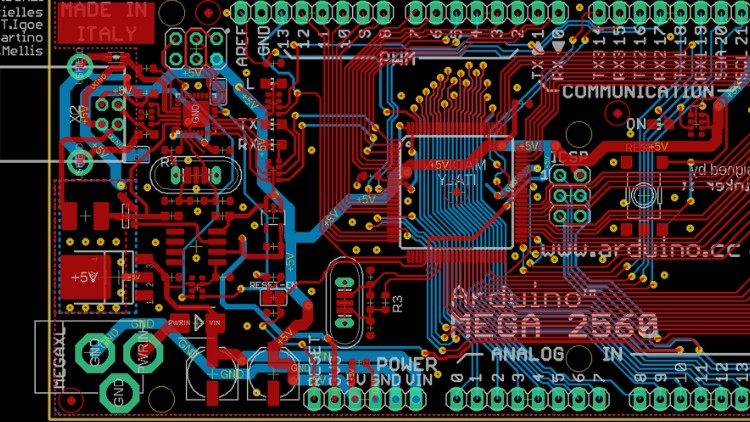
\includegraphics[width=8cm]{imagenes/img2} \label{subfiguraA}}
\subfigure[]{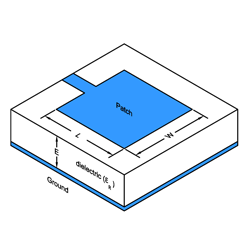
\includegraphics[width=4cm]{imagenes/img3} \label{subfiguraB}}
\subfigure[]{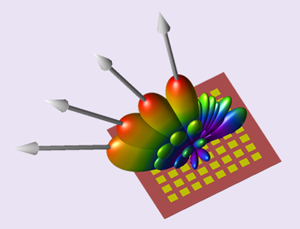
\includegraphics[width=4cm]{imagenes/img4} \label{subfiguraC}}
\caption{Tenemos tres subfiguras, la subfigura \ref{subfiguraA}, tambien tenemos la \ref{subfiguraB} y la \ref{subfiguraC}}
\label{3figs}
\end{figure}

\subsubsection{Tablas}
las tablas tambien son importantes, y estas se enumerarán como en la tabla \eqref{tabla1}
\begin{table}
\caption{Unidades para las propiedades MAgnéticas} %%CPonemos nuestra descripción al encabezado de las tablas
\label{tabla1} %etiqueta de \begin{table}...\end{table}
\setlength{\tabcolsep}{3pt}%separacion del texto de la tabla (3 puntos)
\begin{tabular}{|p{25pt}|p{75pt}|p{115pt}|} %las lineas verticales se inclyen con el comando "|", y las medidas, o ancho de cada columna de dan en puntos "pt" o lo pueden hacer en centimetros, no excediendo los 8.5cm, hacer la prueba
\hline % nos ofrece lineas horizontales
Sym            & Quantity                               & Conversion from Gaussian and \par CGS EMU to SI $^{\mathrm{a}}$ \\
\hline
$\Phi $        & magnetic flux                          & 1 Mx $\to  10^{-8}$ Wb $= 10^{-8}$ V$\cdot $s \\
$B$            & magnetic flux density, magnetic induction    & 1 G $\to  10^{-4}$ T $= 10^{-4}$ Wb/m$^{2}$ \\
$H$            & magnetic field strength                & 1 Oe $\to  10^{3}/(4\pi )$ A/m \\
$m$            & magnetic moment                        & 1 erg/G $=$ 1 emu \par $\to 10^{-3}$ A$\cdot $m$^{2} = 10^{-3}$ J/T \\
$M$            & magnetization                          & 1 erg/(G$\cdot $cm$^{3}) =$ 1 emu/cm$^{3}$ \par $\to 10^{3}$ A/m \\
4$\pi M$       & magnetization                          & 1 G $\to  10^{3}/(4\pi )$ A/m \\
$\sigma $      & specific magnetization                 & 1 erg/(G$\cdot $g) $=$ 1 emu/g $\to $ 1 A$\cdot $m$^{2}$/kg \\
$j$            & magnetic dipole moment                 & 1 erg/G $=$ 1 emu \par $\to 4\pi \times  10^{-10}$ Wb$\cdot $m \\
$J$            & magnetic polarization                  & 1 erg/(G$\cdot $cm$^{3}) =$ 1 emu/cm$^{3}$ \par $\to 4\pi \times  10^{-4}$ T \\
$\chi, \kappa $& susceptibility                        & 1 $\to  4\pi $ \\
$\chi_{\rho }$ & mass susceptibility                    & 1 cm$^{3}$/g $\to  4\pi \times  10^{-3}$ m$^{3}$/kg \\
$\mu $         & permeability                           & 1 $\to  4\pi \times  10^{-7}$ H/m \par $= 4\pi \times  10^{-7}$ Wb/(A$\cdot $m) \\
$\mu_{r}$      & relative permeability                  & $\mu \to \mu_{r}$ \\
$w, W$         & energy density                         & 1 erg/cm$^{3} \to  10^{-1}$ J/m$^{3}$ \\
$N, D$         & demagnetizing factor                   & 1 $\to  1/(4\pi )$ \\
\hline
\multicolumn{3}{p{251pt}}{Tenemos la opción de incluir texto con un ancho que sea igual o parecido al total del inicio para conceptos complementarios.}\\ % se incluye el numero 3, por que queremos abarcar las 3 columnas
\multicolumn{3}{p{251pt}}{$^{\mathrm{a}}$Gaussian units are the same as cg emu for magnetostatics; Mx
$=$ maxwell, G $=$ gauss, Oe $=$ oersted; Wb $=$ weber, V $=$ volt, s $=$
second, T $=$ tesla, m $=$ meter, A $=$ ampere, J $=$ joule, kg $=$
kilogram, H $=$ henry.} %% Abarcamos las 3 columnas, pero sigue siendo parte de la tabla. Podemos encerrarla con lineas laterales, este ejersicio lo dejamos para ustedes, experimenten :p
\end{tabular}
\end{table}

\subsubsection{Otros}

tambien podemos agregar tablas simples, para datos pequeños usando el siguiete comando

\begin{tabular}{ccc}  %% podemos usar c: que significa cumna centrada, r: que es columna a la derecha de "right", l: que es comuna a la izquerda de "left". Estas ajustan el ancho de sus columnas automaticamente, de acuerdo al contenido
\hline
columna1 & columna2 & columna3 \\
\hline
algoA    & algoB    & algoC \\
masA     & mas B    & mas C
\end{tabular}

pero tener presente que estos no se pueden poner etiquetas para referenciarlas, es una manera simple de organizar en tablas

\subsection{Lineas de Código}

Muchas veces tendremos la necesidad de incluir lineas de código los cuales se pueden incluir en partes o completas, de acuerdo a lo que se quiera presentar como sigue de manera completa

\lstinputlisting[language=Octave]{codigo/cod1.m}

o incluirla por partes, seleccionando las lineas que queremos incluir en nuestro informe

\lstinputlisting[language=Octave, firstline=4, lastline=9]{codigo/cod1.m}

Para ello se hace el uso sel package \texttt{listings}. El paquete listings es capaz de resaltar los siguientes lenguajes:

ABAP$^{2,4}$, ACSL, Ada$^4$, Algol$^4$, Ant, Assembler$^{2,4}$, Awk$^4$, bash, Basic$^{2,4}$, C\#$^{5}$, C++$^4$, C$^4$, Caml$^4$, Clean, Cobol$^4$, Comal, csh, Delphi, Eiffel, Elan, erlang, Euphoria, Fortran$^4$, GCL, Gnuplot, Haskell, HTML, IDL$^4$, inform, Java$^4$, JVMIS, ksh, Lisp$^4$, Logo, Lua$^2$, make$^4$, Mathematica$^{1,4}$, Matlab, Mercury, MetaPost, Miranda, Mizar, ML, Modelica$^3$, Modula-2, MuPAD, NASTRAN, Oberon-2, Objective C$^5$ , OCL$^4$, Octave, Oz, Pascal$^4$, Perl, PHP, PL/I, Plasm, POV, Prolog, Promela, Python, R, Reduce, Rexx, RSL, Ruby, S$^4$, SAS, Scilab, sh, SHELXL, Simula$^4$, SQL, tcl$^4$, TeX4, VBScript, Verilog, VHDL$^4$, VRML$^4$, XML, XSLT.

\begin{enumerate}
\item Soporta Mathematica solamente si se trata de un fichero en texto plano. No se pueden incluir ficheros *.NB., sin embargo, Mathematica puede exportar ficheros fuente formateados para su uso en \LaTeX.
\item En estos lenguajes es obligatorio especificar el dialecto del lenguaje (por ejemplo: \texttt{language={[x86masm]Assembler}}).
\item Modelica se soporta mediante el paquete \texttt{dtsyntax} disponible en \url{https://code.google.com/archive/p/dtsyntax/}
\item Para estos lenguajes hay múltiples dialectos soportados: C, por ejemplo, puede ser ANSI, Handel, Objective y Sharp. Ver p. 12 del \url{http://ctan.dcc.uchile.cl/macros/latex/contrib/listings/listings.pdf} para una introducción a esto.
\item Definido como un dialecto de otro lenguaje.
\end{enumerate}

%%%%%%%%%%%%%%%%%%%%%%%%%%%%%%%%%%%%%%%%%%%%%%%
%%%%%
%%%%%   CONCLUSIONES     %%%%%%%%%%%%%%%%%%%%%%
%%%%%
%%%%%%%%%%%%%%%%%%%%%%%%%%%%%%%%%%%%%%%%%%%%%%%

\section{Conclusiones}
A conclusion section is not required. Although a conclusion may review the
main points of the paper, do not replicate the abstract as the conclusion. A
conclusion might elaborate on the importance of the work or suggest
applications and extensions.

%%%%%%%%%%%%%%%%%%%%%%%%%%%%%%%%%%%%%%%%%%%%%%%
%%%%%
%%%%%   BIBLIOGRAFÍA     %%%%%%%%%%%%%%%%%%%%%%
%%%%%
%%%%%%%%%%%%%%%%%%%%%%%%%%%%%%%%%%%%%%%%%%%%%%%

\bibliographystyle{ieeetr}
\bibliography{bibliografia}

\end{document}
